\documentclass[11pt]{article}

    \usepackage[breakable]{tcolorbox}
    \usepackage{parskip} % Stop auto-indenting (to mimic markdown behaviour)
    

    % Basic figure setup, for now with no caption control since it's done
    % automatically by Pandoc (which extracts ![](path) syntax from Markdown).
    \usepackage{graphicx}
    % Keep aspect ratio if custom image width or height is specified
    \setkeys{Gin}{keepaspectratio}
    % Maintain compatibility with old templates. Remove in nbconvert 6.0
    \let\Oldincludegraphics\includegraphics
    % Ensure that by default, figures have no caption (until we provide a
    % proper Figure object with a Caption API and a way to capture that
    % in the conversion process - todo).
    \usepackage{caption}
    \DeclareCaptionFormat{nocaption}{}
    \captionsetup{format=nocaption,aboveskip=0pt,belowskip=0pt}

    \usepackage{float}
    \floatplacement{figure}{H} % forces figures to be placed at the correct location
    \usepackage{xcolor} % Allow colors to be defined
    \usepackage{enumerate} % Needed for markdown enumerations to work
    \usepackage{geometry} % Used to adjust the document margins
    \usepackage{amsmath} % Equations
    \usepackage{amssymb} % Equations
    \usepackage{textcomp} % defines textquotesingle
    % Hack from http://tex.stackexchange.com/a/47451/13684:
    \AtBeginDocument{%
        \def\PYZsq{\textquotesingle}% Upright quotes in Pygmentized code
    }
    \usepackage{upquote} % Upright quotes for verbatim code
    \usepackage{eurosym} % defines \euro

    \usepackage{iftex}
    \ifPDFTeX
        \usepackage[T1]{fontenc}
        \IfFileExists{alphabeta.sty}{
              \usepackage{alphabeta}
          }{
              \usepackage[mathletters]{ucs}
              \usepackage[utf8x]{inputenc}
          }
    \else
        \usepackage{fontspec}
        \usepackage{unicode-math}
    \fi

    \usepackage{fancyvrb} % verbatim replacement that allows latex
    \usepackage{grffile} % extends the file name processing of package graphics
                         % to support a larger range
    \makeatletter % fix for old versions of grffile with XeLaTeX
    \@ifpackagelater{grffile}{2019/11/01}
    {
      % Do nothing on new versions
    }
    {
      \def\Gread@@xetex#1{%
        \IfFileExists{"\Gin@base".bb}%
        {\Gread@eps{\Gin@base.bb}}%
        {\Gread@@xetex@aux#1}%
      }
    }
    \makeatother
    \usepackage[Export]{adjustbox} % Used to constrain images to a maximum size
    \adjustboxset{max size={0.9\linewidth}{0.9\paperheight}}

    % The hyperref package gives us a pdf with properly built
    % internal navigation ('pdf bookmarks' for the table of contents,
    % internal cross-reference links, web links for URLs, etc.)
    \usepackage{hyperref}
    % The default LaTeX title has an obnoxious amount of whitespace. By default,
    % titling removes some of it. It also provides customization options.
    \usepackage{titling}
    \usepackage{longtable} % longtable support required by pandoc >1.10
    \usepackage{booktabs}  % table support for pandoc > 1.12.2
    \usepackage{array}     % table support for pandoc >= 2.11.3
    \usepackage{calc}      % table minipage width calculation for pandoc >= 2.11.1
    \usepackage[inline]{enumitem} % IRkernel/repr support (it uses the enumerate* environment)
    \usepackage[normalem]{ulem} % ulem is needed to support strikethroughs (\sout)
                                % normalem makes italics be italics, not underlines
    \usepackage{soul}      % strikethrough (\st) support for pandoc >= 3.0.0
    \usepackage{mathrsfs}
    

    
    % Colors for the hyperref package
    \definecolor{urlcolor}{rgb}{0,.145,.698}
    \definecolor{linkcolor}{rgb}{.71,0.21,0.01}
    \definecolor{citecolor}{rgb}{.12,.54,.11}

    % ANSI colors
    \definecolor{ansi-black}{HTML}{3E424D}
    \definecolor{ansi-black-intense}{HTML}{282C36}
    \definecolor{ansi-red}{HTML}{E75C58}
    \definecolor{ansi-red-intense}{HTML}{B22B31}
    \definecolor{ansi-green}{HTML}{00A250}
    \definecolor{ansi-green-intense}{HTML}{007427}
    \definecolor{ansi-yellow}{HTML}{DDB62B}
    \definecolor{ansi-yellow-intense}{HTML}{B27D12}
    \definecolor{ansi-blue}{HTML}{208FFB}
    \definecolor{ansi-blue-intense}{HTML}{0065CA}
    \definecolor{ansi-magenta}{HTML}{D160C4}
    \definecolor{ansi-magenta-intense}{HTML}{A03196}
    \definecolor{ansi-cyan}{HTML}{60C6C8}
    \definecolor{ansi-cyan-intense}{HTML}{258F8F}
    \definecolor{ansi-white}{HTML}{C5C1B4}
    \definecolor{ansi-white-intense}{HTML}{A1A6B2}
    \definecolor{ansi-default-inverse-fg}{HTML}{FFFFFF}
    \definecolor{ansi-default-inverse-bg}{HTML}{000000}

    % common color for the border for error outputs.
    \definecolor{outerrorbackground}{HTML}{FFDFDF}

    % commands and environments needed by pandoc snippets
    % extracted from the output of `pandoc -s`
    \providecommand{\tightlist}{%
      \setlength{\itemsep}{0pt}\setlength{\parskip}{0pt}}
    \DefineVerbatimEnvironment{Highlighting}{Verbatim}{commandchars=\\\{\}}
    % Add ',fontsize=\small' for more characters per line
    \newenvironment{Shaded}{}{}
    \newcommand{\KeywordTok}[1]{\textcolor[rgb]{0.00,0.44,0.13}{\textbf{{#1}}}}
    \newcommand{\DataTypeTok}[1]{\textcolor[rgb]{0.56,0.13,0.00}{{#1}}}
    \newcommand{\DecValTok}[1]{\textcolor[rgb]{0.25,0.63,0.44}{{#1}}}
    \newcommand{\BaseNTok}[1]{\textcolor[rgb]{0.25,0.63,0.44}{{#1}}}
    \newcommand{\FloatTok}[1]{\textcolor[rgb]{0.25,0.63,0.44}{{#1}}}
    \newcommand{\CharTok}[1]{\textcolor[rgb]{0.25,0.44,0.63}{{#1}}}
    \newcommand{\StringTok}[1]{\textcolor[rgb]{0.25,0.44,0.63}{{#1}}}
    \newcommand{\CommentTok}[1]{\textcolor[rgb]{0.38,0.63,0.69}{\textit{{#1}}}}
    \newcommand{\OtherTok}[1]{\textcolor[rgb]{0.00,0.44,0.13}{{#1}}}
    \newcommand{\AlertTok}[1]{\textcolor[rgb]{1.00,0.00,0.00}{\textbf{{#1}}}}
    \newcommand{\FunctionTok}[1]{\textcolor[rgb]{0.02,0.16,0.49}{{#1}}}
    \newcommand{\RegionMarkerTok}[1]{{#1}}
    \newcommand{\ErrorTok}[1]{\textcolor[rgb]{1.00,0.00,0.00}{\textbf{{#1}}}}
    \newcommand{\NormalTok}[1]{{#1}}

    % Additional commands for more recent versions of Pandoc
    \newcommand{\ConstantTok}[1]{\textcolor[rgb]{0.53,0.00,0.00}{{#1}}}
    \newcommand{\SpecialCharTok}[1]{\textcolor[rgb]{0.25,0.44,0.63}{{#1}}}
    \newcommand{\VerbatimStringTok}[1]{\textcolor[rgb]{0.25,0.44,0.63}{{#1}}}
    \newcommand{\SpecialStringTok}[1]{\textcolor[rgb]{0.73,0.40,0.53}{{#1}}}
    \newcommand{\ImportTok}[1]{{#1}}
    \newcommand{\DocumentationTok}[1]{\textcolor[rgb]{0.73,0.13,0.13}{\textit{{#1}}}}
    \newcommand{\AnnotationTok}[1]{\textcolor[rgb]{0.38,0.63,0.69}{\textbf{\textit{{#1}}}}}
    \newcommand{\CommentVarTok}[1]{\textcolor[rgb]{0.38,0.63,0.69}{\textbf{\textit{{#1}}}}}
    \newcommand{\VariableTok}[1]{\textcolor[rgb]{0.10,0.09,0.49}{{#1}}}
    \newcommand{\ControlFlowTok}[1]{\textcolor[rgb]{0.00,0.44,0.13}{\textbf{{#1}}}}
    \newcommand{\OperatorTok}[1]{\textcolor[rgb]{0.40,0.40,0.40}{{#1}}}
    \newcommand{\BuiltInTok}[1]{{#1}}
    \newcommand{\ExtensionTok}[1]{{#1}}
    \newcommand{\PreprocessorTok}[1]{\textcolor[rgb]{0.74,0.48,0.00}{{#1}}}
    \newcommand{\AttributeTok}[1]{\textcolor[rgb]{0.49,0.56,0.16}{{#1}}}
    \newcommand{\InformationTok}[1]{\textcolor[rgb]{0.38,0.63,0.69}{\textbf{\textit{{#1}}}}}
    \newcommand{\WarningTok}[1]{\textcolor[rgb]{0.38,0.63,0.69}{\textbf{\textit{{#1}}}}}
    \makeatletter
    \newsavebox\pandoc@box
    \newcommand*\pandocbounded[1]{%
      \sbox\pandoc@box{#1}%
      % scaling factors for width and height
      \Gscale@div\@tempa\textheight{\dimexpr\ht\pandoc@box+\dp\pandoc@box\relax}%
      \Gscale@div\@tempb\linewidth{\wd\pandoc@box}%
      % select the smaller of both
      \ifdim\@tempb\p@<\@tempa\p@
        \let\@tempa\@tempb
      \fi
      % scaling accordingly (\@tempa < 1)
      \ifdim\@tempa\p@<\p@
        \scalebox{\@tempa}{\usebox\pandoc@box}%
      % scaling not needed, use as it is
      \else
        \usebox{\pandoc@box}%
      \fi
    }
    \makeatother

    % Define a nice break command that doesn't care if a line doesn't already
    % exist.
    \def\br{\hspace*{\fill} \\* }
    % Math Jax compatibility definitions
    \def\gt{>}
    \def\lt{<}
    \let\Oldtex\TeX
    \let\Oldlatex\LaTeX
    \renewcommand{\TeX}{\textrm{\Oldtex}}
    \renewcommand{\LaTeX}{\textrm{\Oldlatex}}
    % Document parameters
    % Document title
    \title{05\_notes}
    
    
    
    
    
    
    
% Pygments definitions
\makeatletter
\def\PY@reset{\let\PY@it=\relax \let\PY@bf=\relax%
    \let\PY@ul=\relax \let\PY@tc=\relax%
    \let\PY@bc=\relax \let\PY@ff=\relax}
\def\PY@tok#1{\csname PY@tok@#1\endcsname}
\def\PY@toks#1+{\ifx\relax#1\empty\else%
    \PY@tok{#1}\expandafter\PY@toks\fi}
\def\PY@do#1{\PY@bc{\PY@tc{\PY@ul{%
    \PY@it{\PY@bf{\PY@ff{#1}}}}}}}
\def\PY#1#2{\PY@reset\PY@toks#1+\relax+\PY@do{#2}}

\@namedef{PY@tok@w}{\def\PY@tc##1{\textcolor[rgb]{0.73,0.73,0.73}{##1}}}
\@namedef{PY@tok@c}{\let\PY@it=\textit\def\PY@tc##1{\textcolor[rgb]{0.24,0.48,0.48}{##1}}}
\@namedef{PY@tok@cp}{\def\PY@tc##1{\textcolor[rgb]{0.61,0.40,0.00}{##1}}}
\@namedef{PY@tok@k}{\let\PY@bf=\textbf\def\PY@tc##1{\textcolor[rgb]{0.00,0.50,0.00}{##1}}}
\@namedef{PY@tok@kp}{\def\PY@tc##1{\textcolor[rgb]{0.00,0.50,0.00}{##1}}}
\@namedef{PY@tok@kt}{\def\PY@tc##1{\textcolor[rgb]{0.69,0.00,0.25}{##1}}}
\@namedef{PY@tok@o}{\def\PY@tc##1{\textcolor[rgb]{0.40,0.40,0.40}{##1}}}
\@namedef{PY@tok@ow}{\let\PY@bf=\textbf\def\PY@tc##1{\textcolor[rgb]{0.67,0.13,1.00}{##1}}}
\@namedef{PY@tok@nb}{\def\PY@tc##1{\textcolor[rgb]{0.00,0.50,0.00}{##1}}}
\@namedef{PY@tok@nf}{\def\PY@tc##1{\textcolor[rgb]{0.00,0.00,1.00}{##1}}}
\@namedef{PY@tok@nc}{\let\PY@bf=\textbf\def\PY@tc##1{\textcolor[rgb]{0.00,0.00,1.00}{##1}}}
\@namedef{PY@tok@nn}{\let\PY@bf=\textbf\def\PY@tc##1{\textcolor[rgb]{0.00,0.00,1.00}{##1}}}
\@namedef{PY@tok@ne}{\let\PY@bf=\textbf\def\PY@tc##1{\textcolor[rgb]{0.80,0.25,0.22}{##1}}}
\@namedef{PY@tok@nv}{\def\PY@tc##1{\textcolor[rgb]{0.10,0.09,0.49}{##1}}}
\@namedef{PY@tok@no}{\def\PY@tc##1{\textcolor[rgb]{0.53,0.00,0.00}{##1}}}
\@namedef{PY@tok@nl}{\def\PY@tc##1{\textcolor[rgb]{0.46,0.46,0.00}{##1}}}
\@namedef{PY@tok@ni}{\let\PY@bf=\textbf\def\PY@tc##1{\textcolor[rgb]{0.44,0.44,0.44}{##1}}}
\@namedef{PY@tok@na}{\def\PY@tc##1{\textcolor[rgb]{0.41,0.47,0.13}{##1}}}
\@namedef{PY@tok@nt}{\let\PY@bf=\textbf\def\PY@tc##1{\textcolor[rgb]{0.00,0.50,0.00}{##1}}}
\@namedef{PY@tok@nd}{\def\PY@tc##1{\textcolor[rgb]{0.67,0.13,1.00}{##1}}}
\@namedef{PY@tok@s}{\def\PY@tc##1{\textcolor[rgb]{0.73,0.13,0.13}{##1}}}
\@namedef{PY@tok@sd}{\let\PY@it=\textit\def\PY@tc##1{\textcolor[rgb]{0.73,0.13,0.13}{##1}}}
\@namedef{PY@tok@si}{\let\PY@bf=\textbf\def\PY@tc##1{\textcolor[rgb]{0.64,0.35,0.47}{##1}}}
\@namedef{PY@tok@se}{\let\PY@bf=\textbf\def\PY@tc##1{\textcolor[rgb]{0.67,0.36,0.12}{##1}}}
\@namedef{PY@tok@sr}{\def\PY@tc##1{\textcolor[rgb]{0.64,0.35,0.47}{##1}}}
\@namedef{PY@tok@ss}{\def\PY@tc##1{\textcolor[rgb]{0.10,0.09,0.49}{##1}}}
\@namedef{PY@tok@sx}{\def\PY@tc##1{\textcolor[rgb]{0.00,0.50,0.00}{##1}}}
\@namedef{PY@tok@m}{\def\PY@tc##1{\textcolor[rgb]{0.40,0.40,0.40}{##1}}}
\@namedef{PY@tok@gh}{\let\PY@bf=\textbf\def\PY@tc##1{\textcolor[rgb]{0.00,0.00,0.50}{##1}}}
\@namedef{PY@tok@gu}{\let\PY@bf=\textbf\def\PY@tc##1{\textcolor[rgb]{0.50,0.00,0.50}{##1}}}
\@namedef{PY@tok@gd}{\def\PY@tc##1{\textcolor[rgb]{0.63,0.00,0.00}{##1}}}
\@namedef{PY@tok@gi}{\def\PY@tc##1{\textcolor[rgb]{0.00,0.52,0.00}{##1}}}
\@namedef{PY@tok@gr}{\def\PY@tc##1{\textcolor[rgb]{0.89,0.00,0.00}{##1}}}
\@namedef{PY@tok@ge}{\let\PY@it=\textit}
\@namedef{PY@tok@gs}{\let\PY@bf=\textbf}
\@namedef{PY@tok@ges}{\let\PY@bf=\textbf\let\PY@it=\textit}
\@namedef{PY@tok@gp}{\let\PY@bf=\textbf\def\PY@tc##1{\textcolor[rgb]{0.00,0.00,0.50}{##1}}}
\@namedef{PY@tok@go}{\def\PY@tc##1{\textcolor[rgb]{0.44,0.44,0.44}{##1}}}
\@namedef{PY@tok@gt}{\def\PY@tc##1{\textcolor[rgb]{0.00,0.27,0.87}{##1}}}
\@namedef{PY@tok@err}{\def\PY@bc##1{{\setlength{\fboxsep}{\string -\fboxrule}\fcolorbox[rgb]{1.00,0.00,0.00}{1,1,1}{\strut ##1}}}}
\@namedef{PY@tok@kc}{\let\PY@bf=\textbf\def\PY@tc##1{\textcolor[rgb]{0.00,0.50,0.00}{##1}}}
\@namedef{PY@tok@kd}{\let\PY@bf=\textbf\def\PY@tc##1{\textcolor[rgb]{0.00,0.50,0.00}{##1}}}
\@namedef{PY@tok@kn}{\let\PY@bf=\textbf\def\PY@tc##1{\textcolor[rgb]{0.00,0.50,0.00}{##1}}}
\@namedef{PY@tok@kr}{\let\PY@bf=\textbf\def\PY@tc##1{\textcolor[rgb]{0.00,0.50,0.00}{##1}}}
\@namedef{PY@tok@bp}{\def\PY@tc##1{\textcolor[rgb]{0.00,0.50,0.00}{##1}}}
\@namedef{PY@tok@fm}{\def\PY@tc##1{\textcolor[rgb]{0.00,0.00,1.00}{##1}}}
\@namedef{PY@tok@vc}{\def\PY@tc##1{\textcolor[rgb]{0.10,0.09,0.49}{##1}}}
\@namedef{PY@tok@vg}{\def\PY@tc##1{\textcolor[rgb]{0.10,0.09,0.49}{##1}}}
\@namedef{PY@tok@vi}{\def\PY@tc##1{\textcolor[rgb]{0.10,0.09,0.49}{##1}}}
\@namedef{PY@tok@vm}{\def\PY@tc##1{\textcolor[rgb]{0.10,0.09,0.49}{##1}}}
\@namedef{PY@tok@sa}{\def\PY@tc##1{\textcolor[rgb]{0.73,0.13,0.13}{##1}}}
\@namedef{PY@tok@sb}{\def\PY@tc##1{\textcolor[rgb]{0.73,0.13,0.13}{##1}}}
\@namedef{PY@tok@sc}{\def\PY@tc##1{\textcolor[rgb]{0.73,0.13,0.13}{##1}}}
\@namedef{PY@tok@dl}{\def\PY@tc##1{\textcolor[rgb]{0.73,0.13,0.13}{##1}}}
\@namedef{PY@tok@s2}{\def\PY@tc##1{\textcolor[rgb]{0.73,0.13,0.13}{##1}}}
\@namedef{PY@tok@sh}{\def\PY@tc##1{\textcolor[rgb]{0.73,0.13,0.13}{##1}}}
\@namedef{PY@tok@s1}{\def\PY@tc##1{\textcolor[rgb]{0.73,0.13,0.13}{##1}}}
\@namedef{PY@tok@mb}{\def\PY@tc##1{\textcolor[rgb]{0.40,0.40,0.40}{##1}}}
\@namedef{PY@tok@mf}{\def\PY@tc##1{\textcolor[rgb]{0.40,0.40,0.40}{##1}}}
\@namedef{PY@tok@mh}{\def\PY@tc##1{\textcolor[rgb]{0.40,0.40,0.40}{##1}}}
\@namedef{PY@tok@mi}{\def\PY@tc##1{\textcolor[rgb]{0.40,0.40,0.40}{##1}}}
\@namedef{PY@tok@il}{\def\PY@tc##1{\textcolor[rgb]{0.40,0.40,0.40}{##1}}}
\@namedef{PY@tok@mo}{\def\PY@tc##1{\textcolor[rgb]{0.40,0.40,0.40}{##1}}}
\@namedef{PY@tok@ch}{\let\PY@it=\textit\def\PY@tc##1{\textcolor[rgb]{0.24,0.48,0.48}{##1}}}
\@namedef{PY@tok@cm}{\let\PY@it=\textit\def\PY@tc##1{\textcolor[rgb]{0.24,0.48,0.48}{##1}}}
\@namedef{PY@tok@cpf}{\let\PY@it=\textit\def\PY@tc##1{\textcolor[rgb]{0.24,0.48,0.48}{##1}}}
\@namedef{PY@tok@c1}{\let\PY@it=\textit\def\PY@tc##1{\textcolor[rgb]{0.24,0.48,0.48}{##1}}}
\@namedef{PY@tok@cs}{\let\PY@it=\textit\def\PY@tc##1{\textcolor[rgb]{0.24,0.48,0.48}{##1}}}

\def\PYZbs{\char`\\}
\def\PYZus{\char`\_}
\def\PYZob{\char`\{}
\def\PYZcb{\char`\}}
\def\PYZca{\char`\^}
\def\PYZam{\char`\&}
\def\PYZlt{\char`\<}
\def\PYZgt{\char`\>}
\def\PYZsh{\char`\#}
\def\PYZpc{\char`\%}
\def\PYZdl{\char`\$}
\def\PYZhy{\char`\-}
\def\PYZsq{\char`\'}
\def\PYZdq{\char`\"}
\def\PYZti{\char`\~}
% for compatibility with earlier versions
\def\PYZat{@}
\def\PYZlb{[}
\def\PYZrb{]}
\makeatother


    % For linebreaks inside Verbatim environment from package fancyvrb.
    \makeatletter
        \newbox\Wrappedcontinuationbox
        \newbox\Wrappedvisiblespacebox
        \newcommand*\Wrappedvisiblespace {\textcolor{red}{\textvisiblespace}}
        \newcommand*\Wrappedcontinuationsymbol {\textcolor{red}{\llap{\tiny$\m@th\hookrightarrow$}}}
        \newcommand*\Wrappedcontinuationindent {3ex }
        \newcommand*\Wrappedafterbreak {\kern\Wrappedcontinuationindent\copy\Wrappedcontinuationbox}
        % Take advantage of the already applied Pygments mark-up to insert
        % potential linebreaks for TeX processing.
        %        {, <, #, %, $, ' and ": go to next line.
        %        _, }, ^, &, >, - and ~: stay at end of broken line.
        % Use of \textquotesingle for straight quote.
        \newcommand*\Wrappedbreaksatspecials {%
            \def\PYGZus{\discretionary{\char`\_}{\Wrappedafterbreak}{\char`\_}}%
            \def\PYGZob{\discretionary{}{\Wrappedafterbreak\char`\{}{\char`\{}}%
            \def\PYGZcb{\discretionary{\char`\}}{\Wrappedafterbreak}{\char`\}}}%
            \def\PYGZca{\discretionary{\char`\^}{\Wrappedafterbreak}{\char`\^}}%
            \def\PYGZam{\discretionary{\char`\&}{\Wrappedafterbreak}{\char`\&}}%
            \def\PYGZlt{\discretionary{}{\Wrappedafterbreak\char`\<}{\char`\<}}%
            \def\PYGZgt{\discretionary{\char`\>}{\Wrappedafterbreak}{\char`\>}}%
            \def\PYGZsh{\discretionary{}{\Wrappedafterbreak\char`\#}{\char`\#}}%
            \def\PYGZpc{\discretionary{}{\Wrappedafterbreak\char`\%}{\char`\%}}%
            \def\PYGZdl{\discretionary{}{\Wrappedafterbreak\char`\$}{\char`\$}}%
            \def\PYGZhy{\discretionary{\char`\-}{\Wrappedafterbreak}{\char`\-}}%
            \def\PYGZsq{\discretionary{}{\Wrappedafterbreak\textquotesingle}{\textquotesingle}}%
            \def\PYGZdq{\discretionary{}{\Wrappedafterbreak\char`\"}{\char`\"}}%
            \def\PYGZti{\discretionary{\char`\~}{\Wrappedafterbreak}{\char`\~}}%
        }
        % Some characters . , ; ? ! / are not pygmentized.
        % This macro makes them "active" and they will insert potential linebreaks
        \newcommand*\Wrappedbreaksatpunct {%
            \lccode`\~`\.\lowercase{\def~}{\discretionary{\hbox{\char`\.}}{\Wrappedafterbreak}{\hbox{\char`\.}}}%
            \lccode`\~`\,\lowercase{\def~}{\discretionary{\hbox{\char`\,}}{\Wrappedafterbreak}{\hbox{\char`\,}}}%
            \lccode`\~`\;\lowercase{\def~}{\discretionary{\hbox{\char`\;}}{\Wrappedafterbreak}{\hbox{\char`\;}}}%
            \lccode`\~`\:\lowercase{\def~}{\discretionary{\hbox{\char`\:}}{\Wrappedafterbreak}{\hbox{\char`\:}}}%
            \lccode`\~`\?\lowercase{\def~}{\discretionary{\hbox{\char`\?}}{\Wrappedafterbreak}{\hbox{\char`\?}}}%
            \lccode`\~`\!\lowercase{\def~}{\discretionary{\hbox{\char`\!}}{\Wrappedafterbreak}{\hbox{\char`\!}}}%
            \lccode`\~`\/\lowercase{\def~}{\discretionary{\hbox{\char`\/}}{\Wrappedafterbreak}{\hbox{\char`\/}}}%
            \catcode`\.\active
            \catcode`\,\active
            \catcode`\;\active
            \catcode`\:\active
            \catcode`\?\active
            \catcode`\!\active
            \catcode`\/\active
            \lccode`\~`\~
        }
    \makeatother

    \let\OriginalVerbatim=\Verbatim
    \makeatletter
    \renewcommand{\Verbatim}[1][1]{%
        %\parskip\z@skip
        \sbox\Wrappedcontinuationbox {\Wrappedcontinuationsymbol}%
        \sbox\Wrappedvisiblespacebox {\FV@SetupFont\Wrappedvisiblespace}%
        \def\FancyVerbFormatLine ##1{\hsize\linewidth
            \vtop{\raggedright\hyphenpenalty\z@\exhyphenpenalty\z@
                \doublehyphendemerits\z@\finalhyphendemerits\z@
                \strut ##1\strut}%
        }%
        % If the linebreak is at a space, the latter will be displayed as visible
        % space at end of first line, and a continuation symbol starts next line.
        % Stretch/shrink are however usually zero for typewriter font.
        \def\FV@Space {%
            \nobreak\hskip\z@ plus\fontdimen3\font minus\fontdimen4\font
            \discretionary{\copy\Wrappedvisiblespacebox}{\Wrappedafterbreak}
            {\kern\fontdimen2\font}%
        }%

        % Allow breaks at special characters using \PYG... macros.
        \Wrappedbreaksatspecials
        % Breaks at punctuation characters . , ; ? ! and / need catcode=\active
        \OriginalVerbatim[#1,codes*=\Wrappedbreaksatpunct]%
    }
    \makeatother

    % Exact colors from NB
    \definecolor{incolor}{HTML}{303F9F}
    \definecolor{outcolor}{HTML}{D84315}
    \definecolor{cellborder}{HTML}{CFCFCF}
    \definecolor{cellbackground}{HTML}{F7F7F7}

    % prompt
    \makeatletter
    \newcommand{\boxspacing}{\kern\kvtcb@left@rule\kern\kvtcb@boxsep}
    \makeatother
    \newcommand{\prompt}[4]{
        {\ttfamily\llap{{\color{#2}[#3]:\hspace{3pt}#4}}\vspace{-\baselineskip}}
    }
    

    
    % Prevent overflowing lines due to hard-to-break entities
    \sloppy
    % Setup hyperref package
    \hypersetup{
      breaklinks=true,  % so long urls are correctly broken across lines
      colorlinks=true,
      urlcolor=urlcolor,
      linkcolor=linkcolor,
      citecolor=citecolor,
      }
    % Slightly bigger margins than the latex defaults
    
    \geometry{verbose,tmargin=1in,bmargin=1in,lmargin=1in,rmargin=1in}
    
    

\begin{document}
    
    \maketitle
    
    

    
    \section{Week 5 - Notes: Conservation of
Energy}\label{week-5---notes-conservation-of-energy}

One expression of a conservation law is the
\href{https://en.wikipedia.org/wiki/Conservation_of_energy}{conservation
of energy}. For an isolated and closed system, the total energy is
conserved. That is, before and after any process, we can account for all
the energy in the system and it is the same. More generally,
conservation of energy accounts for the energy ``lost'' to the
surroundings. All of the changes to the system must be accounted for in
changes the surroundings.

For a given choice of system that interacts with its surroundings, the
change in energy of the system is equal to the work done on the system
and any heat exchanged with the surroundings. This is a statement of the
\href{https://en.wikipedia.org/wiki/First_law_of_thermodynamics}{first
law of thermodynamics}. We can write that statement mathematically as:

\[\Delta E_{\text{system}} = W + Q\]

where \(\Delta E_{\text{system}}\) is the change in energy of the
system, \(W\) is the work done on the system, and \(Q\) is the heat
exchanged with the surroundings.

:::\{admonition\} Sign conventions :class: warning

Note that the signs of the work done and heat exchanged are important.
But we can remember them by asking if the system is going to increase
its energy.

If we add energy into the system by heating it, then \(Q\) is positive
because \(\Delta E_{\text{system}}\) is positive. If the remove energy
from the system through an exchange of heat, then \(Q\) is negative.

If the system does work on the surroundings, for example, by exerting a
force on an external object over some displacement, then \(W\) is
negative because \(\Delta E_{\text{system}}\) is negative. If instead
the surroundings do work on the system, then \(W\) is positive.

:::

We can rewrite this energy equation as an update equation for the energy
of the system:

\[E_{\text{system,f}} = E_{\text{system,i}} + W + Q\]

From this equation, we can see that the final state of the system's
energy is determined by the sum of its initial energy, the work done on
the system, and the heat exchanged with the surroundings.

    \subsection{The Work-Energy Theorem}\label{the-work-energy-theorem}

We often model a system as a single object that interacts with its
surroundings. In this case, it's often beneficial to select the object
alone to be the system of interest. Then all of our work is to explain
and predict the dynamics of the object.

This simplification allows us to employ a more specialized case of the
general energy equation. We can write the work-energy theorem as:

\[\Delta E_{\text{object}} = W_{\text{net}}\] where
\(\Delta E_{\text{object}}\) is the change in energy of the object and
\(W_{\text{net}}\) is the net work done on the object.

More specifically, we often focus only on the changes to the object's
motion. This is because we use often use the model of a
\href{https://en.wikipedia.org/wiki/Point_particle}{point particle} to
describe the object. In this case, the object has no internal structure
and thus no internal energy. The only energy we need to consider is the
object's kinetic energy, \(K\).

:::\{admonition\} Limitation of this model

The point particle model where we focus on the kinetic energy of an
object is an obvious simplification. But it might not be so obvious how
quickly it is to break down.

Consider pushing a block across the floor. The block is a point particle
and we model it as such. It comes to a stop and we argue the block's
kinetic energy was converted to heat in the floor.

But what about the block itself? Would it's surface temperature
increase? It does, but we don't account for it.

A great account of these kinds of situations is from my colleague
\href{https:/brucesherwood.net/}{Bruce Sherwood}. Bruce's paper,
\href{https://pubs.aip.org/aapt/ajp/article-abstract/51/7/597/1052185/Pseudowork-and-real-work?redirectedFrom=fulltext}{\emph{Pseudowork
and real work}, American Journal of Physics (1982)}, is an important
read about the limitation of the point particle model. You can find a
PDF copy
\href{https://brucesherwood.net/wp-content/uploads/2017/06/Pseudowork1983.pdf}{here}.
:::

    \subsubsection{Kinetic Energy}\label{kinetic-energy}

Our model of \href{https://en.wikipedia.org/wiki/Kinetic_energy}{kinetic
energy} stems from a
\href{https://en.wikipedia.org/wiki/Willem_\%27s_Gravesande}{series of
experiments dropping stones into clay}. The depth of the hole made was
proportional to the square of the impact speed.

Through many additional experiments we have quantified the kinetic
energy of a point particle as:

\[K = \frac{1}{2}m\vec{v}\cdot\vec{v}.\]

We also use \(T\) to represent kinetic energy, so you might see it
written as:

\[T = \frac{1}{2}mv^2.\]

Note that this description of the kinetic energy is fully classical. It
is the energy of motion in the limit that object moves much slower than
the speed of light. We learned from
\href{https://en.wikipedia.org/wiki/Special_theory_of_relativity}{Einstein's
special theory of relativity} that the total energy of an point particle
is:

\[E_{tot} = \gamma mc^2,\]

where \(\gamma\) is the
\href{https://en.wikipedia.org/wiki/Lorentz_factor}{Lorentz factor} and
\(c\) is the speed of light. The Lorentz factor is defined as:

\[\gamma = \frac{1}{\sqrt{1 - \frac{v^2}{c^2}}}.\]

Notice that if \(v/c =0\) then,

\[\gamma = 1 \longrightarrow E_{tot} = mc^2.\]

We call this the ``rest energy'' of the object. It is the energy of the
object when it is not moving, and it demonstrates the
\href{https://en.wikipedia.org/wiki/Mass\%E2\%80\%93energy_equivalence}{mass-energy
equivalence}.

\[E_{rest} = mc^2.\]

The remaining energy of the object is the kinetic energy, \(T\). We can
write that as:

\[T = E_{tot} - E_{rest} = (\gamma - 1)mc^2.\]

We can take the limit that \(v/c \ll 1\) and expand the Lorentz factor
in a Taylor series to find that:

\[\gamma = 1 + \frac{1}{2}\frac{v^2}{c^2} + \ldots.\]

Then we find that the kinetic energy is:

\[T = \left(1 + \frac{1}{2}\frac{v^2}{c^2} + \ldots - 1\right)mc^2 = \frac{1}{2}mv^2 + \ldots.\]

We have recovered the classical expression for kinetic energy. The
higher order terms in the expansion are negligible when \(v/c \ll 1\).

    \subsection{Developing the Work-Energy
Theorem}\label{developing-the-work-energy-theorem}

Let's start with our definition of the classical kinetic energy of a
point particle:

\[T = \frac{1}{2}m\vec{v}\cdot\vec{v}.\]

We ask how does \(T\) change with time? We take the time derivative of
\(T\):

\[\dfrac{dT}{dt} = \frac{1}{2}m\frac{d}{dt}\left(\vec{v}\cdot\vec{v}\right) = \frac{1}{2}m\left(\frac{d\vec{v}}{dt}\cdot\vec{v} + \vec{v}\cdot\frac{d\vec{v}}{dt}\right).\]

The last term can be combined because the dot product is commutative. We
can factor out the \(m/2\) and write:

\[\dfrac{dT}{dt} = \dfrac{m}{2}\left(2 \dfrac{d\vec{v}}{dt}\cdot\vec{v}\right) = m\left(\dfrac{d\vec{v}}{dt}\cdot\vec{v}\right).\]

Ok, in that expression is the net force on the object,

\[\vec{F}_{net} = m\dfrac{d\vec{v}}{dt}.\]

So that,

\[\dfrac{dT}{dt} = \vec{F}_{net}\cdot\vec{v}.\]

Now let's discretize the time derivative to make sense of this.

\[\dfrac{\Delta T}{\Delta t} = \vec{F}_{net}\cdot\vec{v}.\]

\[\Delta T = \vec{F}_{net}\cdot\vec{v}\Delta t.\]

That last term is the displacement of the object,
\(\Delta \vec{x} = \vec{v}\Delta t\). So we can write:

\[\Delta T = \vec{F}_{net}\cdot\Delta \vec{x}.\]

This is the work done on the object by the net force. We can write that
as:

\[\Delta T = W_{\text{net}}.\]

    \subsubsection{Overall Effect of the
Forces}\label{overall-effect-of-the-forces}

Consider that we are looking at the changes in the object's motion over
a longer period of space and time. This discrete model above helps us
understand the relationship between the work done on the object and the
change in its kinetic energy in a small interval, but what about the
overall effect of the forces on the object?

Consider a discrete set of \(n\) spatial intervals, \(\Delta x_i\),
where \(i\) is the index of the interval.

\[x = {x_0, x_1, x_2, \ldots, x_n}\]

At each of these spatial intervals, we experience a different net force,
like in the figure below.

\begin{figure}
\centering
\pandocbounded{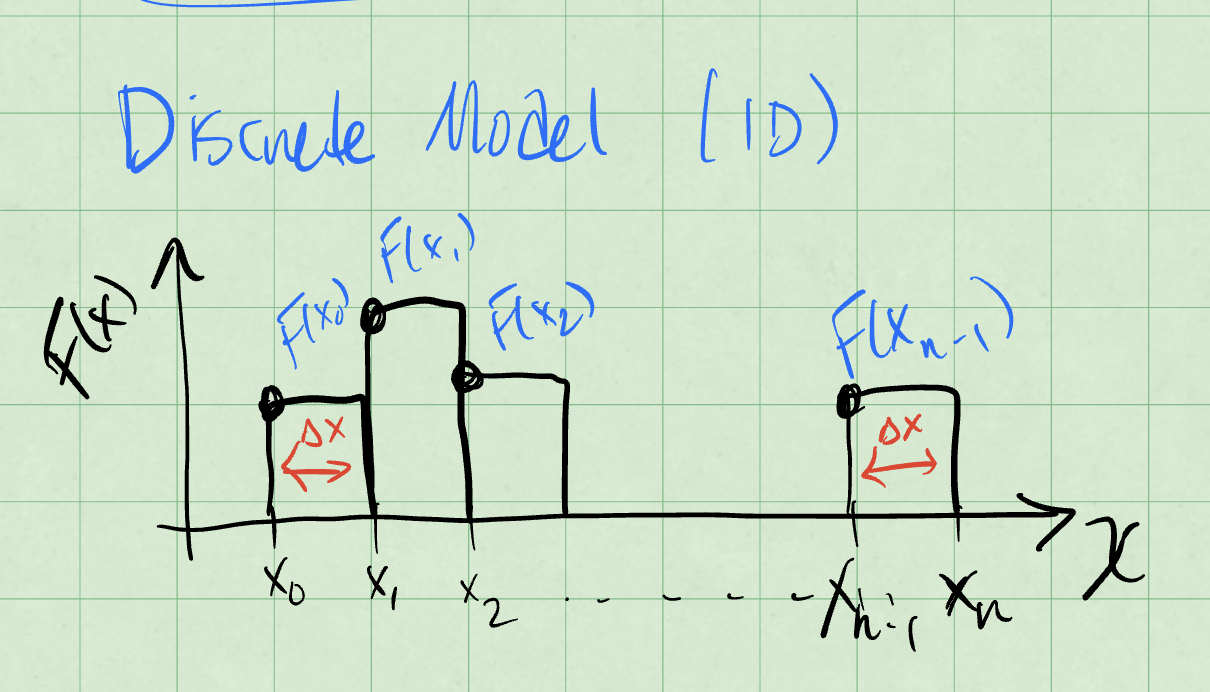
\includegraphics[keepaspectratio,alt={Work done by a net force}]{/Users/caballero/repos/teaching/modern-classical-mechanics/content/images/notes/week5/discrete-force-intervals.png}}
\caption{Work done by a net force}
\end{figure}

\[F_{net} = {F_{net,0}, F_{net,1}, F_{net,2}, \ldots, F_{net,n}}\]

The work done by this force is the change in kinetic energy of the
object:

\[W_{\text{net}} = \sum_{i=0}^{n} F_{net,i}\Delta x_i = \Delta T.\]

\[W_{\text{net}} = K_f - K_i.\]

\[W_{\text{net}} = \dfrac{1}{2}m\vec{v}_f\cdot\vec{v}_f - \dfrac{1}{2}m\vec{v}_i\cdot\vec{v}_i.\]

Notice that in the limit that \(n \rightarrow \infty\) and
\(\Delta x_i \rightarrow 0\), we have a continuous function of the net
force. We can write that as:

\[\lim_{n \rightarrow \infty} \sum_{i=0}^{n} F_{net,i}\Delta x_i = \int_{x_i}^{x_f} F_{net}(x)dx.\]

Thus, in our continuous limit, we can write the work done by the net
force as:

\[\Delta T = W_{\text{net}} = \int_{x_i}^{x_f} F_{net}(x)dx.\]

What about in more than one dimension?

    \subsubsection{Work done in more than one
dimension}\label{work-done-in-more-than-one-dimension}

Consider a path \(C\) that we have discretized into \(n\) intervals. The
object starts at \(\vec{r}_0\) and ends at \(\vec{r}_n\). Each interval
is \(\Delta \vec{r}_i\) and the net force is \(\vec{F}_{net,i}\). The
figure below shows the work done by the net force in each interval.

\begin{figure}
\centering
\pandocbounded{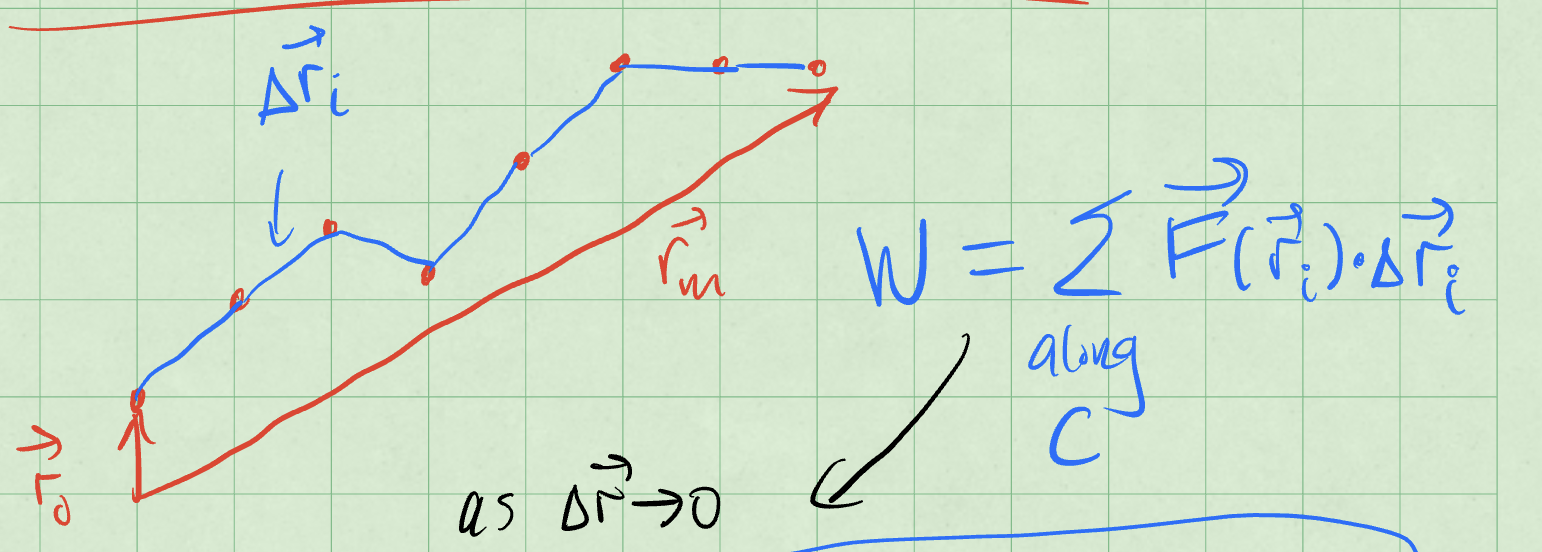
\includegraphics[keepaspectratio,alt={Work done by a net force}]{/Users/caballero/repos/teaching/modern-classical-mechanics/content/images/notes/week5/path-integral-work.png}}
\caption{Work done by a net force}
\end{figure}

The work done by the net force is:

\[W_{\text{net}} = \sum_{i=0}^{n} \vec{F}_{net,i}\cdot\Delta \vec{r}_i.\]

as \(\Delta \vec{r}_i \rightarrow 0\) and \(n \rightarrow \infty\), we
have a continuous function of the net force. We can write that as:

\[W_{\text{net}} = \int_{C} \vec{F}_{net}\cdot d\vec{r}.\]

The work can be positive, if the force and displacement are in the same
direction, or negative, if they are in opposite directions. It can also
be zero, if the force is perpendicular to the displacement.

If the force is \textbf{always} perpendicular to the displacement, then
the work done by the force is zero. This is because the dot product of
two perpendicular vectors is zero. But what kind of motion is possible?

    \subsection{Example: The Simple Harmonic
Oscillator}\label{example-the-simple-harmonic-oscillator}

Consider, again, the humble
\href{https://en.wikipedia.org/wiki/Harmonic_oscillator}{SHO}. If we
have a horizontal spring mass system, we know we can write the force on
the mass as:

\[F_s = -kx.\]

Let's allow the spring to move from \(x_i\) to \(x_f\), while the speed
changes from \(v_i\) to \(v_f\).

The change in kinetic energy is:

\[\Delta T = \dfrac{1}{2}mv_f^2 - \dfrac{1}{2}mv_i^2.\]

The work done by the spring is:

\[W_s = \int_{x_i}^{x_f} F_s dx = -\int_{x_i}^{x_f} kx dx = -\left[\dfrac{1}{2}kx^2\right]_{x_i}^{x_f} = -\left(\dfrac{1}{2}kx_f^2 - \dfrac{1}{2}kx_i^2\right).\]

Or more simply,

\[W_s = \dfrac{1}{2}k(x_i^2 - x_f^2).\]

The Work-Energy Theorem tells us that:

\[\Delta T = W_s.\]

\[\dfrac{1}{2}mv_f^2 - \dfrac{1}{2}mv_i^2 = \dfrac{1}{2}k(x_i^2 - x_f^2).\]

We can rearrange this to find the relationship between the states before
and after the motion:

\[\dfrac{1}{2}mv_f^2 + \dfrac{1}{2}k x_f^2 = \dfrac{1}{2}mv_i^2 + \dfrac{1}{2}k x_i^2.\]

The first term on the left and right side are the energy due to motion.
The second terms are some other energy, but taken together before and
after the motion, they are the same. They are a constant. \textbf{This
is a
\href{https://en.wikipedia.org/wiki/Mass\%E2\%80\%93energy_equivalence\#Conservation_of_mass_and_energy}{conserved
quantity}.}

We call the second quantity the \textbf{potential energy} of the
spring-mass system. It is the energy of the system due to its position,
or it's ``configuration''. We define the potential energy of the spring
as:

\[U_s = \dfrac{1}{2}kx^2.\]

We often use \(V\) to represent potential energy, so you might see it
written as:

\[V_s = \dfrac{1}{2}kx^2.\]

What we have discovered is that the total energy of the spring-mass
system is:

\[E_{tot} = T + U_s = \dfrac{1}{2}mv^2 + \dfrac{1}{2}kx^2 = \text{constant}.\]

You have likely seen this previously in your study of the SHO. It is a
very important result. But it is also the case that we don't always have
a potential energy function.

We need to have a
\href{https://en.wikipedia.org/wiki/Conservative_force}{conservative
force} to have a potential energy function. A conservative force is one
where the work done by the force is independent of the path taken.
Above, we assumed that in our calculations because the force was only
dependent on the position of the object. That is a key feature of a
conservative force.

    \subsection{Example: A Lattice Chain}\label{example-a-lattice-chain}

A less obivous example that produces a potential energy function is a
\href{https://en.wikipedia.org/wiki/Lattice_chain}{lattice chain}. Here
we model an electron moving in 1D near but not too near a long chain of
atoms. The picture below shows the model.

\begin{figure}
\centering
\pandocbounded{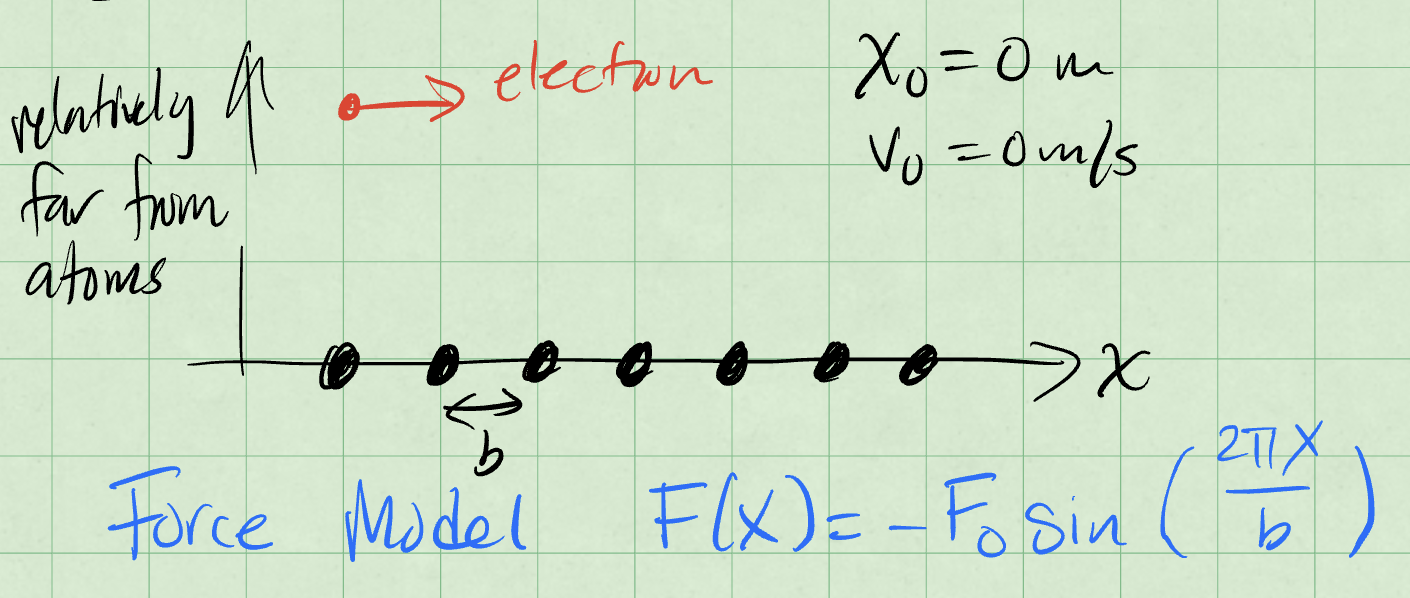
\includegraphics[keepaspectratio,alt={Lattice chain model}]{/Users/caballero/repos/teaching/modern-classical-mechanics/content/images/notes/week5/lattice-chain.png}}
\caption{Lattice chain model}
\end{figure}

Here the location of the particle and it's initial velocty are zero. The
force model for a chain of atoms in this arrangement is:

\[F(x) = -F_0 \sin \left(\dfrac{2\pi x}{b}\right)\]

where \(b\) is the spacing between the atoms and \(F_0\) is a constant.

We can again find the kinetic energy change and work done by the force:

\[\Delta T = \dfrac{1}{2}mv_f^2 - \dfrac{1}{2}mv_i^2 = \dfrac{1}{2}mv_f^2.\]

\[W = \int_{0}^{x_f} F(x) dx = -F_0 \int_{0}^{x_f} \sin \left(\dfrac{2\pi x}{b}\right) dx = -\left[-\dfrac{b}{2\pi}F_0 \cos \left(\dfrac{2\pi x}{b}\right)\right]_{0}^{x_f}\]

\[ = \dfrac{b}{2\pi}F_0 \left(\cos \left(\dfrac{2\pi x_f}{b}\right) - \cos \left(0\right)\right).\]

Using the Work-Energy Theorem, we can write:

\[\dfrac{1}{2}mv_f^2 = \dfrac{b}{2\pi}F_0 \left(\cos \left(\dfrac{2\pi x_f}{b}\right) - 1\right).\]

Thus, we can find the speed of the object at a given position:

\[v_f(x) = \sqrt{\dfrac{b}{\pi m}F_0 \left(\cos \left(\dfrac{2\pi x_f}{b}\right) - 1\right)}.\]

But more importantly, we can derive a potential energy function for the
lattice chain. We can write:

\[U(x) = -\int F(x) dx = \dfrac{b}{2\pi}F_0 \cos \left(\dfrac{2\pi x}{b}\right) + C.\]
where \(C\) is a constant. We can choose \(C\) so that \(U(0) = 0\);
only the difference in potential energy matter. Then we have:

\[U(x) = \dfrac{b}{2\pi}F_0 \cos \left(\dfrac{2\pi x}{b}\right).\]

This is just \textbf{another} conservative force.

    \subsection{Conservative Forces}\label{conservative-forces}

These forces occur frequently enough in physics and their properties are
so important that they deserve their own attention. There are a few key
properties of conservative forces that we should note:

\begin{enumerate}
\def\labelenumi{\arabic{enumi}.}
\tightlist
\item
  if the work is independent of the path taken, then the force is
  conservative.
\item
  if the work done by the force is zero for a closed path, then the
  force is conservative.
\item
  if the curl of the force is zero, then the force is conservative.
\end{enumerate}

It turns out that all of these statements are equivalent. And if any one
of them is true, the rest hold, and we can develop a potential energy
function for the force.

\subsubsection{Why do these imply each
other?}\label{why-do-these-imply-each-other}

Let's start with the curl of the force. The
\href{https://en.wikipedia.org/wiki/Curl}{curl} of a vector field is a
measure of the rotation of the field. It is a
\href{https://en.wikipedia.org/wiki/Vector_calculus_operator}{vector
differential operator}. Operationally, taking the curl amounts to a
cross product of the del operator with the vector field. The curl of a
vector field \(\vec{F}\) is defined as:

\[\nabla \times \vec{F} = \begin{vmatrix}\hat{i} & \hat{j} & \hat{k} \\ \partial_x & \partial_y & \partial_z \\ F_x & F_y & F_z \end{vmatrix} = \left(\dfrac{\partial F_z}{\partial y} - \dfrac{\partial F_y}{\partial z}\right)\hat{i} + \left(\dfrac{\partial F_x}{\partial z} - \dfrac{\partial F_z}{\partial x}\right)\hat{j} + \left(\dfrac{\partial F_y}{\partial x} - \dfrac{\partial F_x}{\partial y}\right)\hat{k}.\]

In the event that the curl vanishes, we know that each term in the curl
is zero. In this case, we can investigate what this implies about other
aspects of the force. We write
\href{https://en.wikipedia.org/wiki/Stokes\%27_theorem}{Stokes' theorem}
for the force as:

\[\iint_S (\nabla \times \vec{F})\cdot d\vec{S} = \oint_C \vec{F}\cdot d\vec{r}.\]

The left hand side is the integral of the curl of the force over some
surface \(S\) with boundary \(C\). The right hand side is the line
integral of the force around the boundary of the surface. This theorem
holds for any vector field with continuous first derivatives, so most of
what we do.

Stokes's theorem tells us that for any choice of surface \(S\) with
boundary \(C\), the line integral of the force around the boundary is
equal to the integral of the curl of the force over the surface. If the
curl vanishes, then the integral of the curl is zero. Thus, the line
integral of the force around the boundary is zero.

\[\oint_C \vec{F}\cdot d\vec{r} = 0.\]

This is true for any closed path \(C\). This is the second statement
above.

We can equivalent write the integral of the force around a closed path
as the work around a different path. The figure below shows these paths
\(C_1\) and \(C_2\) that make up the first loop, and the paths \(C_3\)
and \(C_4\) that make up the second loop. The work done by the force
along each path is shown in the figure.

\begin{figure}
\centering
\pandocbounded{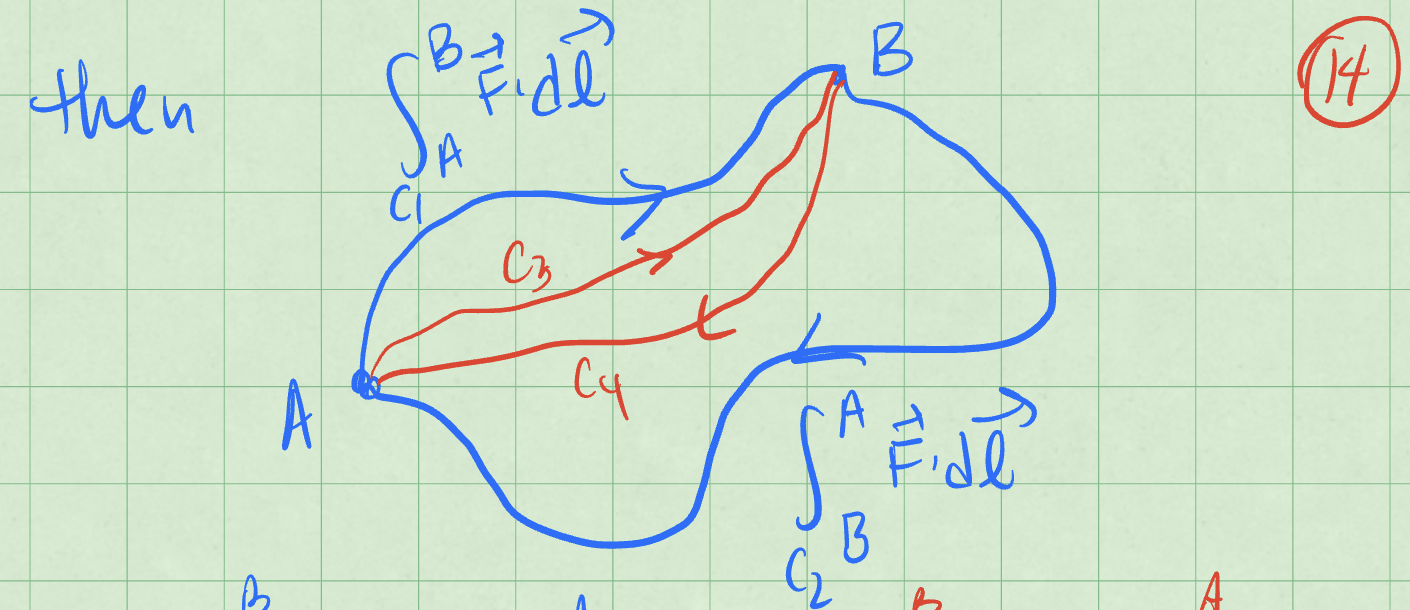
\includegraphics[keepaspectratio,alt={Work done by a net force}]{/Users/caballero/repos/teaching/modern-classical-mechanics/content/images/notes/week5/closed-path-work.png}}
\caption{Work done by a net force}
\end{figure}

We can take the integral of both paths and write:

\[\oint_C \vec{F}\cdot d\vec{r} = \int_{C_1} \vec{F}\cdot d\vec{r} + \int_{C_2} \vec{F}\cdot d\vec{r} = \int_{C_3} \vec{F}\cdot d\vec{r} + \int_{C_4} \vec{F}\cdot d\vec{r} = 0.\]

Because both paths are closed and start and return to the same point, we
can know that each contribution on each part of the path is equal and
opposite. Thus, we can write:

\[\int_{C_n} \vec{F}\cdot d\vec{r} = -\int_{C_m} \vec{F}\cdot d\vec{r}.\]

This holds for any \(n\) and \(m\) where they make a closed path \(C\).
This is the first statement above.

    \subsection{Summary of Results}\label{summary-of-results}

We covered a lot fo ground. Let's remind ourselves of the key results.

The total energy of a system is the sum of the kinetic and potential
energies:

\[E = T + V = K +U.\]

We use both \(T\) and \(K\) to represent kinetic energy, and both \(U\)
and \(V\) to represent potential energy.

The conservation of energy is:

\[\dfrac{dE}{dt} = 0.\]

When all the forces are conservative, energy is conserved. Of course, we
are limiting here to mechanical energy.

Conservative forces are those where the work done by the force is
independent of the path taken. They have several key properties:

\begin{enumerate}
\def\labelenumi{\arabic{enumi}.}
\tightlist
\item
  The forces are functions of position only \(\vec{F}(\vec{r})\).
\item
  Their curl is zero: \(\nabla \times \vec{F} = 0\).
\end{enumerate}

We calculate the curl as:
\[\nabla \times \vec{F} = \begin{vmatrix}\hat{i} & \hat{j} & \hat{k} \\ \partial_x & \partial_y & \partial_z \\ F_x & F_y & F_z \end{vmatrix} = \left(\dfrac{\partial F_z}{\partial y} - \dfrac{\partial F_y}{\partial z}\right)\hat{i} + \left(\dfrac{\partial F_x}{\partial z} - \dfrac{\partial F_z}{\partial x}\right)\hat{j} + \left(\dfrac{\partial F_y}{\partial x} - \dfrac{\partial F_x}{\partial y}\right)\hat{k}.\]

\begin{enumerate}
\def\labelenumi{\arabic{enumi}.}
\setcounter{enumi}{2}
\tightlist
\item
  The force is given by the negative gradient of the potential energy:
  \(\vec{F} = -\nabla U\). This stems from the definition of the
  potential energy as the work done by the force.
\end{enumerate}

We can calculate the gradient as:

\[\vec{F} = \langle F_x, F_y, F_z \rangle = -\nabla U = -\left(\dfrac{\partial U}{\partial x}\hat{i} + \dfrac{\partial U}{\partial y}\hat{j} + \dfrac{\partial U}{\partial z}\hat{k}\right).\]

\begin{enumerate}
\def\labelenumi{\arabic{enumi}.}
\setcounter{enumi}{3}
\tightlist
\item
  The work done by a conservative force is path independent. We can
  write the work done by a conservative force as:
\end{enumerate}

\[W = \int_{C} \vec{F}\cdot d\vec{r} = -\int_{C} \nabla U\cdot d\vec{r} = -\Delta U.\]

    


    % Add a bibliography block to the postdoc
    
    
    
\end{document}
